% Options for packages loaded elsewhere
% Options for packages loaded elsewhere
\PassOptionsToPackage{unicode}{hyperref}
\PassOptionsToPackage{hyphens}{url}
\PassOptionsToPackage{dvipsnames,svgnames,x11names}{xcolor}
%
\documentclass[
  10pt,
  twocolumn]{article}
\usepackage{xcolor}
\usepackage[top=0.68in,bottom=0.65in,left=0.82in,right=0.82in]{geometry}
\usepackage{amsmath,amssymb}
\setcounter{secnumdepth}{-\maxdimen} % remove section numbering
\usepackage{iftex}
\ifPDFTeX
  \usepackage[T1]{fontenc}
  \usepackage[utf8]{inputenc}
  \usepackage{textcomp} % provide euro and other symbols
\else % if luatex or xetex
  \usepackage{unicode-math} % this also loads fontspec
  \defaultfontfeatures{Scale=MatchLowercase}
  \defaultfontfeatures[\rmfamily]{Ligatures=TeX,Scale=1}
\fi
\usepackage{lmodern}
\ifPDFTeX\else
  % xetex/luatex font selection
\fi
% Use upquote if available, for straight quotes in verbatim environments
\IfFileExists{upquote.sty}{\usepackage{upquote}}{}
\IfFileExists{microtype.sty}{% use microtype if available
  \usepackage[]{microtype}
  \UseMicrotypeSet[protrusion]{basicmath} % disable protrusion for tt fonts
}{}
\makeatletter
\@ifundefined{KOMAClassName}{% if non-KOMA class
  \IfFileExists{parskip.sty}{%
    \usepackage{parskip}
  }{% else
    \setlength{\parindent}{0pt}
    \setlength{\parskip}{6pt plus 2pt minus 1pt}}
}{% if KOMA class
  \KOMAoptions{parskip=half}}
\makeatother
% Make \paragraph and \subparagraph free-standing
\makeatletter
\ifx\paragraph\undefined\else
  \let\oldparagraph\paragraph
  \renewcommand{\paragraph}{
    \@ifstar
      \xxxParagraphStar
      \xxxParagraphNoStar
  }
  \newcommand{\xxxParagraphStar}[1]{\oldparagraph*{#1}\mbox{}}
  \newcommand{\xxxParagraphNoStar}[1]{\oldparagraph{#1}\mbox{}}
\fi
\ifx\subparagraph\undefined\else
  \let\oldsubparagraph\subparagraph
  \renewcommand{\subparagraph}{
    \@ifstar
      \xxxSubParagraphStar
      \xxxSubParagraphNoStar
  }
  \newcommand{\xxxSubParagraphStar}[1]{\oldsubparagraph*{#1}\mbox{}}
  \newcommand{\xxxSubParagraphNoStar}[1]{\oldsubparagraph{#1}\mbox{}}
\fi
\makeatother


\usepackage{longtable,booktabs,array}
\newcounter{none} % for unnumbered tables
\usepackage{calc} % for calculating minipage widths
% Correct order of tables after \paragraph or \subparagraph
\usepackage{etoolbox}
\makeatletter
\patchcmd\longtable{\par}{\if@noskipsec\mbox{}\fi\par}{}{}
\makeatother
% Allow footnotes in longtable head/foot
\IfFileExists{footnotehyper.sty}{\usepackage{footnotehyper}}{\usepackage{footnote}}
\makesavenoteenv{longtable}
\usepackage{graphicx}
\makeatletter
\newsavebox\pandoc@box
\newcommand*\pandocbounded[1]{% scales image to fit in text height/width
  \sbox\pandoc@box{#1}%
  \Gscale@div\@tempa{\textheight}{\dimexpr\ht\pandoc@box+\dp\pandoc@box\relax}%
  \Gscale@div\@tempb{\linewidth}{\wd\pandoc@box}%
  \ifdim\@tempb\p@<\@tempa\p@\let\@tempa\@tempb\fi% select the smaller of both
  \ifdim\@tempa\p@<\p@\scalebox{\@tempa}{\usebox\pandoc@box}%
  \else\usebox{\pandoc@box}%
  \fi%
}
% Set default figure placement to htbp
\def\fps@figure{htbp}
\makeatother


% definitions for citeproc citations
\NewDocumentCommand\citeproctext{}{}
\NewDocumentCommand\citeproc{mm}{%
  \begingroup\def\citeproctext{#2}\cite{#1}\endgroup}
\makeatletter
 % allow citations to break across lines
 \let\@cite@ofmt\@firstofone
 % avoid brackets around text for \cite:
 \def\@biblabel#1{}
 \def\@cite#1#2{{#1\if@tempswa , #2\fi}}
\makeatother
\newlength{\cslhangindent}
\setlength{\cslhangindent}{1.5em}
\newlength{\csllabelwidth}
\setlength{\csllabelwidth}{3em}
\newenvironment{CSLReferences}[2] % #1 hanging-indent, #2 entry-spacing
 {\begin{list}{}{%
  \setlength{\itemindent}{0pt}
  \setlength{\leftmargin}{0pt}
  \setlength{\parsep}{0pt}
  % turn on hanging indent if param 1 is 1
  \ifodd #1
   \setlength{\leftmargin}{\cslhangindent}
   \setlength{\itemindent}{-1\cslhangindent}
  \fi
  % set entry spacing
  \setlength{\itemsep}{#2\baselineskip}}}
 {\end{list}}
\usepackage{calc}
\newcommand{\CSLBlock}[1]{\hfill\break\parbox[t]{\linewidth}{\strut\ignorespaces#1\strut}}
\newcommand{\CSLLeftMargin}[1]{\parbox[t]{\csllabelwidth}{\strut#1\strut}}
\newcommand{\CSLRightInline}[1]{\parbox[t]{\linewidth - \csllabelwidth}{\strut#1\strut}}
\newcommand{\CSLIndent}[1]{\hspace{\cslhangindent}#1}



\setlength{\emergencystretch}{3em} % prevent overfull lines

\providecommand{\tightlist}{%
  \setlength{\itemsep}{0pt}\setlength{\parskip}{0pt}}



 


\usepackage{graphicx}
\usepackage{xcolor}
\usepackage{titlesec}
\usepackage{fancyhdr}
\usepackage{lastpage}
\usepackage{newtxtext}
\usepackage{enumitem}
\definecolor{reportred}{HTML}{C8102E}

\setlength{\columnsep}{0.25in}
\setlength{\parindent}{1em}
\setlength{\parskip}{0pt}
\setlength{\headheight}{14pt}
\setlength{\headsep}{18pt}
\linespread{1.0}
\setlist{nosep,leftmargin=*}

\titleformat{\section}
  {\normalfont\bfseries\normalsize}
  {}{0pt}{}
\titlespacing*{\section}{0pt}{9pt}{3pt}

\titleformat{\subsection}
  {\normalfont\bfseries\small}
  {}{0pt}{}
\titlespacing*{\subsection}{0pt}{7pt}{2pt}

\fancypagestyle{body}{
  \fancyhf{}
  \fancyhead[L]{\footnotesize\itshape Ramos. \textit{Survivorship Curves of Sunset Hill Cemetery}}
  \fancyhead[R]{\footnotesize Page \thepage\ of \pageref{LastPage}}
  \renewcommand{\headrulewidth}{0pt}
}
\fancypagestyle{plain}{
  \fancyhf{}
  \fancyhead[L]{\footnotesize\itshape Ramos. \textit{Survivorship Curves of Sunset Hill Cemetery}}
  \fancyhead[R]{\footnotesize Page \thepage\ of \pageref{LastPage}}
  \renewcommand{\headrulewidth}{0pt}
}
\pagestyle{body}
\makeatletter
\@ifpackageloaded{caption}{}{\usepackage{caption}}
\AtBeginDocument{%
\ifdefined\contentsname
  \renewcommand*\contentsname{Table of contents}
\else
  \newcommand\contentsname{Table of contents}
\fi
\ifdefined\listfigurename
  \renewcommand*\listfigurename{List of Figures}
\else
  \newcommand\listfigurename{List of Figures}
\fi
\ifdefined\listtablename
  \renewcommand*\listtablename{List of Tables}
\else
  \newcommand\listtablename{List of Tables}
\fi
\ifdefined\figurename
  \renewcommand*\figurename{Figure}
\else
  \newcommand\figurename{Figure}
\fi
\ifdefined\tablename
  \renewcommand*\tablename{Table}
\else
  \newcommand\tablename{Table}
\fi
}
\@ifpackageloaded{float}{}{\usepackage{float}}
\floatstyle{ruled}
\@ifundefined{c@chapter}{\newfloat{codelisting}{h}{lop}}{\newfloat{codelisting}{h}{lop}[chapter]}
\floatname{codelisting}{Listing}
\newcommand*\listoflistings{\listof{codelisting}{List of Listings}}
\makeatother
\makeatletter
\makeatother
\makeatletter
\@ifpackageloaded{caption}{}{\usepackage{caption}}
\@ifpackageloaded{subcaption}{}{\usepackage{subcaption}}
\makeatother
\usepackage{bookmark}
\IfFileExists{xurl.sty}{\usepackage{xurl}}{} % add URL line breaks if available
\urlstyle{same}
% fallback for those not using the hyperref driver hyperxmp:
\makeatletter
\@ifundefined{xmpquote}{\newcommand{\xmpquote}[1]{#1}}{}
\makeatother
\hypersetup{
  pdftitle={Cemetary Lifespan Report},
  pdfauthor={Joe Ramos},
  colorlinks=true,
  linkcolor={blue},
  filecolor={Maroon},
  citecolor={blue},
  urlcolor={blue},
  pdfcreator={LaTeX via pandoc}}


\title{Cemetary Lifespan Report}
\author{Joe Ramos}
\date{2026-10-15}
\begin{document}
\maketitle


\onecolumn
\begingroup
\thispagestyle{empty}
\sffamily

% Publication line and journal masthead
\noindent
\begin{minipage}[t]{0.66\linewidth}
  \scriptsize
  Ramos. \textit{Survivorship Curves of Sunset Hill Cemetery}
  \hfill (2026) 1:1\\
  Valdosta State University, Ecology and Evolution
\end{minipage}
\hfill
\begin{minipage}[t]{0.30\linewidth}
  \raggedleft
  \large Cemetery Demography\\[-2pt]
  \large BIOL 3250
\end{minipage}

\vspace{0.28in}

% Article-type band
\noindent
\colorbox{reportred}{%
  \parbox{\dimexpr\linewidth-2\fboxsep\relax}{%
    \color{white}
    \textbf{RESEARCH ARTICLE}\hfill
    \textbf{CLASS PROJECT}
  }%
}

\vspace{0.18in}

% Title and author line
\noindent
{\fontsize{23}{27}\selectfont
\textbf{Lifespan is Effected by Sex and Marital Status}\par}

\vspace{0.12in}

\noindent
{\small
Josimar Ramos\textsuperscript
}

\vspace{0.08in}

% Structured abstract
\setlength{\fboxsep}{6pt}
\noindent
\fcolorbox{reportred}{white}{%
  \begin{minipage}{\dimexpr\linewidth-2\fboxsep-2\fboxrule\relax}
    \small

    \textbf{Abstract}

    \vspace{3pt}

    \textbf{Purpose:}
    This project describes lifespan patterns in cemetery records and examines
    variation by sex and marital status. [you can do military service of males or pre- and post- a particular year - default 1930]

    \vspace{3pt}

    \textbf{Methods:}
    Recorded available birth and death information from gravestones
    and classified selected characteristics using evidence visible on the
    stones and in burial arrangements. [Go into much greater detail in the methods section]

    \vspace{3pt}

    \textbf{Results:}
    [Summarize the principal patterns in the class data.]

    \vspace{3pt}

    \textbf{Conclusions:}
    [State what the observed patterns suggest and note limitations. Distinguish
    lifespan in this cemetery sample from population life expectancy.]

    \vspace{3pt}

    \textbf{Keywords:}
    cemetery records; lifespan; survivorship; marital status; historical demography
  \end{minipage}%
}

% Bottom-page author and institutional details
\vfill

\noindent\rule{0.56\linewidth}{0.4pt}

\vspace{3pt}

\noindent
{\scriptsize
\textsuperscript{*}Correspondence: jtramos@valdosta.edu\\
\textsuperscript{1}Department of Biology, Valdosta State University,
Valdosta, Georgia, USA\\
Ecology and Evolution, BIOL 3250, Section B
}

\vspace{0.10in}

\noindent
\begin{minipage}[c]{0.20\linewidth}
  
\includegraphics[width=0.72in]{Valdosta_State_University_seal.png}
\end{minipage}
\endgroup
\twocolumn

\section{Background}\label{background}

Cemetery records provide individual birth and death dates that can be
used to describe lifespan among people represented in a burial ground.
These records are a non-random sample: cemetery access, preservation of
markers, migration, family burial practices, and the choice of graves to
record may all affect which people appear in the dataset. The analyses
below therefore describe the collected sample and should not be treated
as direct estimates of lifespan for an entire town or historical
population.

\section{Hypotheses}\label{hypotheses}

Write each hypothesis before interpreting the figures. State the
expected direction and identify the comparison.

\begin{enumerate}
\def\labelenumi{\arabic{enumi}.}
\tightlist
\item
  \textbf{Sex and lifespan:} I hypothesize that women will have a
  greater lifespan than men due to the fact that women have smarter
  decision making skills.
\end{enumerate}

\section{Methods}\label{methods}

\subsection{Field site and sampling}\label{field-site-and-sampling}

\begin{itemize}
\tightlist
\item
  \textbf{Where did you go?} We went to the Sunset Hill Cemetery in
  Valdosta GA next to Oak Street Parking Deck at VSU on October 8th. We
  wrote down names with their respective birthdate and deathdate.
\item
  \textbf{What date and time of day did you collect records?} October
  8th, 2pm-4pm
\item
  \textbf{What part of the cemetery did you sample?} Southeast portion
  of the graveyard
\item
  \textbf{How did you choose graves?} legible name with birthdates and
  deathdates, at random
\item
  \textbf{How did you handle nearby graves and family plots?}
  Neighboring graves were recorded, family included, no bias.
\end{itemize}

\subsection{Recorded information and variable
definitions}\label{recorded-information-and-variable-definitions}

\begin{itemize}
\tightlist
\item
  \textbf{What information did you record from each marker?} Name,
  Birthdate, Deathdate, sex, merital status, and military status.
\item
  \textbf{How was lifespan calculated?} The age of each person was
  transcribed subtracting the deathdate from the birthdate.
\item
  \textbf{How did you determine marital status?} We determined merital
  status from the graves, which were usually jointed if they were
  married.
\item
  \textbf{How did you determine military service?} Usually the
  gravestone would have their military status if they were drafted.
\item
  \textbf{How did you determine sex or gender?} The gravestone was a big
  indicator on what the deceased was sex wise. (Mother, Father, son,
  etc.)
\item
  \textbf{How were missing, illegible, or ambiguous records handled?} We
  tried to skip any illegible gravestones.
\end{itemize}

\subsection{Dataset and analysis}\label{dataset-and-analysis}

\begin{itemize}
\tightlist
\item
  \textbf{How many records were collected by you?} n = 25
\item
  \textbf{How many records were included in the final analysis?} n = 50
\item
  \textbf{Were records aggregated with the class dataset?} No
\item
  \textbf{What summaries or plots were produced?} The graph showed the
  curve for the lifespan between Male v Female excluding military
  status.
\item
  \textbf{What are the limits of the sample?} Some limits would've been
  incomplete dates, legibleness, condidtion of the stone, etc.
\end{itemize}

\section{Results}\label{results}

The summary table in Figure~\ref{fig-summary} shows substantial
differences in recorded lifespan by sex in this sample. Males had a mean
lifespan of 62.2 years (SD =23 ; n = 410), compared with 71.1 years (SD
= 21.9; n = 342) for females.

\begin{figure*}[t]

\centering{

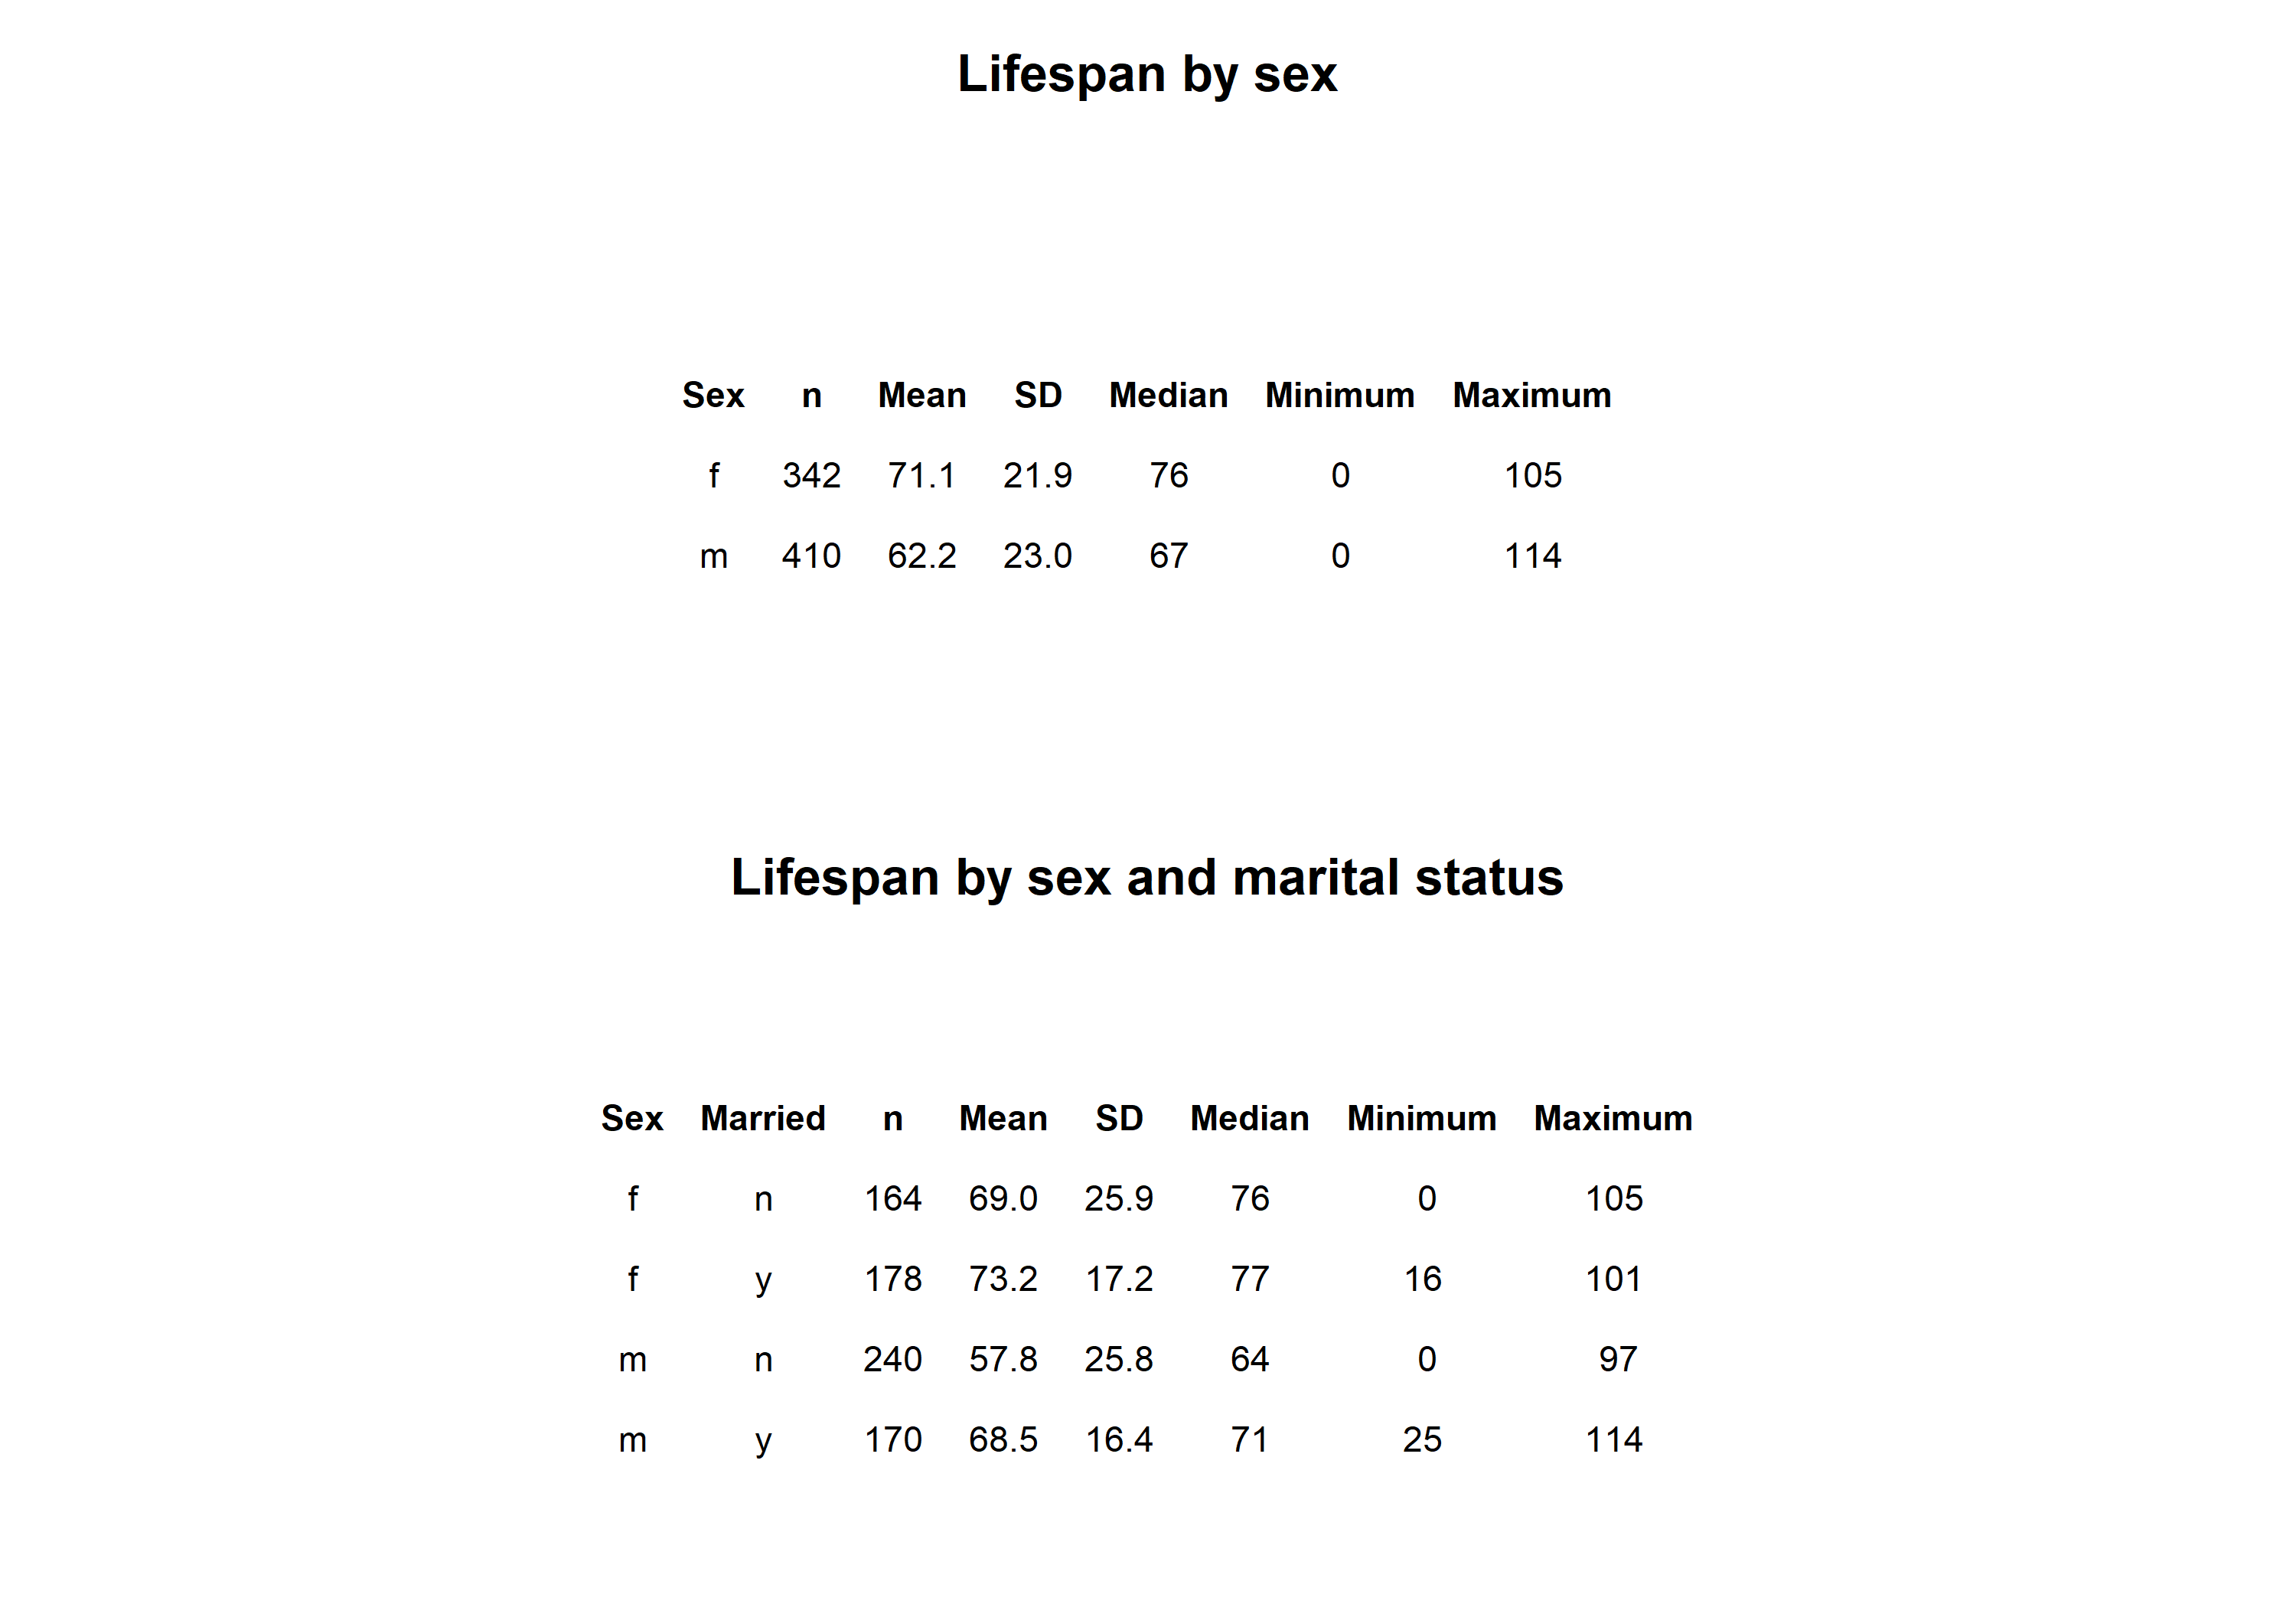
\includegraphics[width=0.9\linewidth,height=\textheight,keepaspectratio]{lifespan_tables/combined_tables.png}

}

\caption{\label{fig-summary}Summary of lifespan by sex}

\end{figure*}%

The sex-specific survivorship curves in Figure~\ref{fig-sex} show a
different pattern: the plotted means are 61.1 years for males and 57.3
years for females. The male curve remains higher through much of the
earlier and middle lifespan, while the female curve reaches the 50\%
survival point later. The curves are close and change relative position,
so the figure suggests that the sex difference depends on which part of
the lifespan distribution is considered. The median markers indicate
where each group's observed curve reaches 50\% surviving; they are
distinct from the mean values shown in the legend.

\begin{figure*}[t]

\centering{

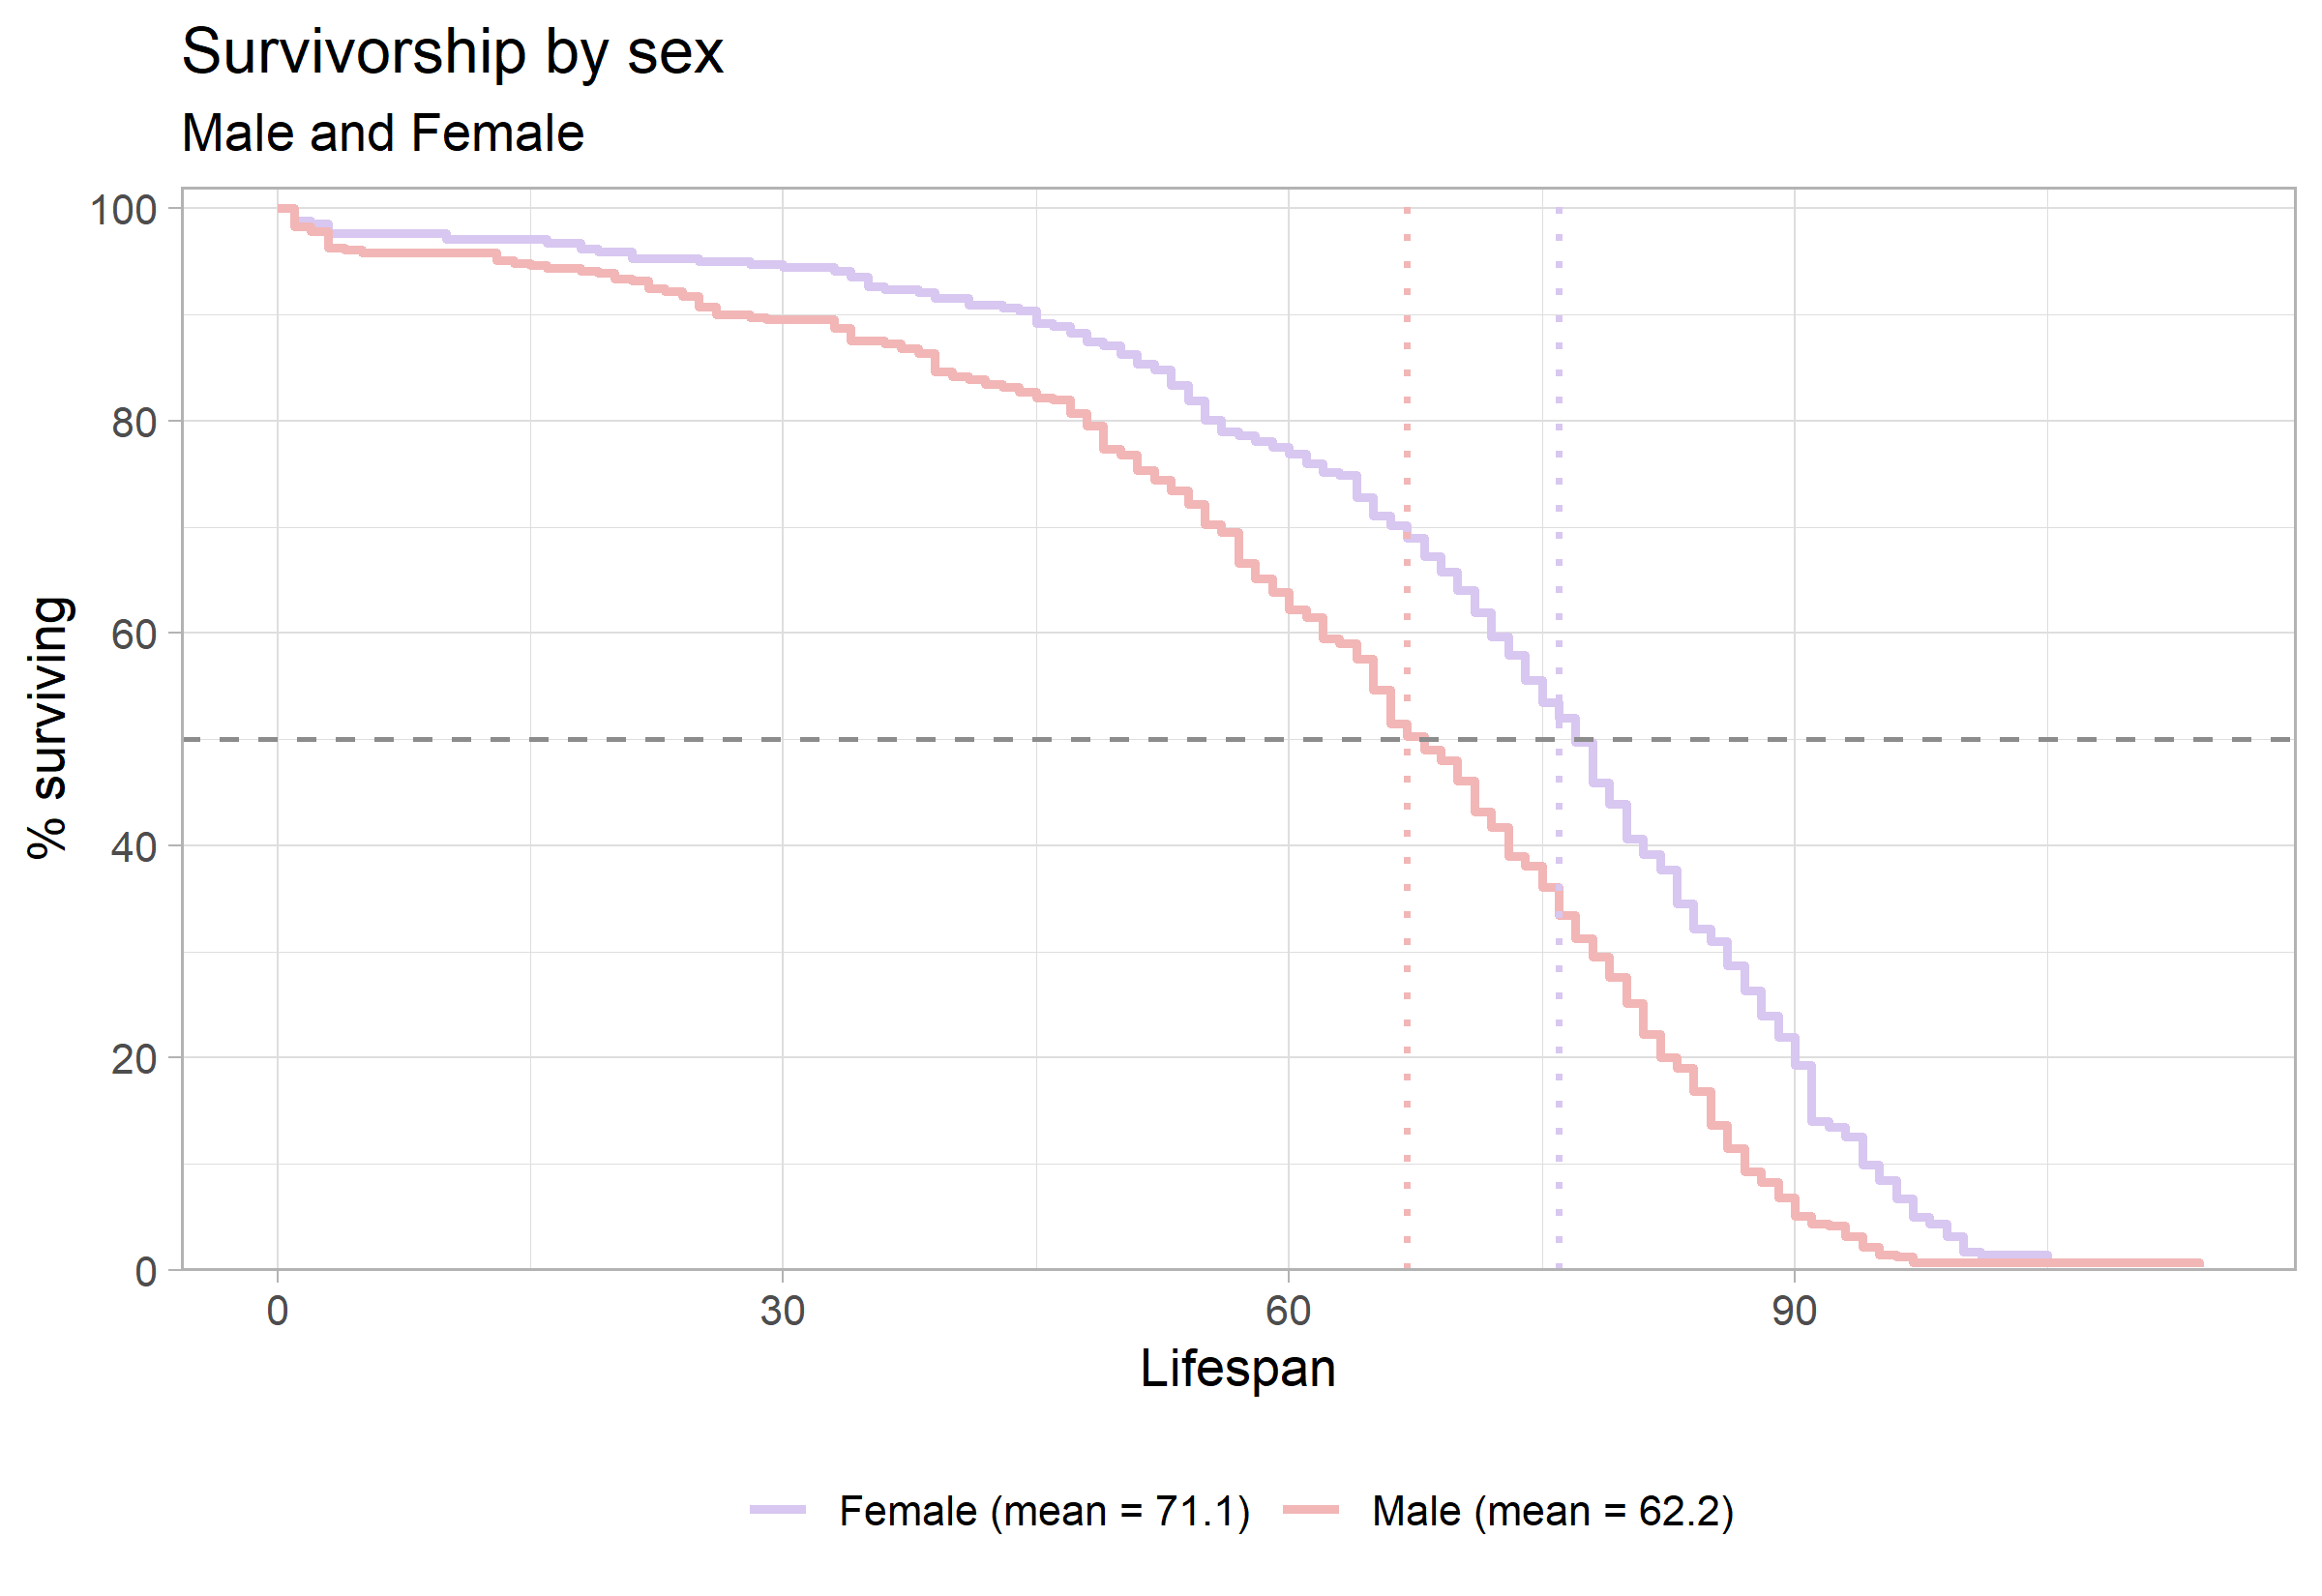
\includegraphics[width=0.7\linewidth,height=\textheight,keepaspectratio]{survivorship_curves/survivorship_by_sex.png}

}

\caption{\label{fig-sex}Survivorship curves by sex. The y-axis shows the
percentage of the cemetery sample surviving to each lifespan. Dotted
vertical lines mark the median lifespan for each sex, where the curve
reaches 50\%.}

\end{figure*}%

\section{Discussion}\label{discussion}

\textbf{Sex and lifespan.} Research on sex differences in longevity
points to a combination of biological, behavioral, and social influences
rather than a single explanation. Austad and Fischer review evidence on
sex differences in lifespan and aging across species, including humans
(Austad \& Fischer, 2016). In this cemetery sample, the observed female
and male curves {[}describe the pattern{]} and {[}support / do not
support{]} the prediction that {[}state your hypothesis{]}. The result
should be interpreted in the context of this cemetery's birth cohorts
and sampling process; it is not by itself an estimate of a general sex
difference in lifespan.

\textbf{Marital status and social relationships.} Marriage can correlate
with social support, health behaviors, household resources, and social
integration, but people's health can also influence whether they marry
or remain married. A large meta-analysis found associations between
unmarried status and mortality, with some associations differing by sex
(Wang \emph{et al.}, 2020); a broader meta-analysis linked social
relationships with mortality risk (Holt-Lunstad \emph{et al.}, 2010). In
this dataset, the comparison of married and not-married records among
{[}men / women / both{]} showed {[}describe results{]}. These cemetery
records do not measure relationship quality, social contact, or the
timing and duration of marriage, so marital status should be treated as
an imperfect indicator rather than a direct measure of socialization or
a cause of longevity.

\textbf{Historical changes in lifespan and childhood survival.} Life
expectancy at birth is strongly affected by deaths in infancy and
childhood, so a low historical average does not mean that every adult
died young. Improvements in clean water and sanitation contributed
substantially to mortality declines in the United States during the
twentieth century, especially for infants and children (Cutler \&
Miller, 2005). The birth-period pattern in this sample {[}describe
results{]} may be consistent with changing survival conditions, but
birth year alone cannot identify which changes mattered. Vaccination,
nutrition, medical care, living conditions, and the incomplete
representation of people in cemetery records may also contribute to
differences across cohorts.

\textbf{Limitations and next steps:} {[}Discuss sample size, missing or
inferred data, cemetery representation, family clustering, survivorship
bias, and what additional evidence would strengthen the analysis.{]}

\newpage

\subsubsection{References}\label{references}

\protect\phantomsection\label{refs}
\begin{CSLReferences}{0}{1}
\bibitem[\citeproctext]{ref-austadSexDifferencesLifespan2016}
\textbf{\textbf{Austad SN}, \textbf{Fischer KE}}. \textbf{2016}.
\href{https://doi.org/10.1016/j.cmet.2016.05.019}{Sex {Differences} in
{Lifespan}}. \emph{Cell Metabolism} \textbf{23}: 1022--1033.

\bibitem[\citeproctext]{ref-cutlerRolePublicHealth2005}
\textbf{\textbf{Cutler D}, \textbf{Miller G}}. \textbf{2005}.
\href{https://doi.org/10.1353/dem.2005.0002}{The role of public health
improvements in health advances: {The} twentieth-century {United
States}}. \emph{Demography} \textbf{42}: 1--22.

\bibitem[\citeproctext]{ref-holt-lunstadSocialRelationshipsMortality2010}
\textbf{\textbf{Holt-Lunstad J}, \textbf{Smith TB}, \textbf{Layton JB}}.
\textbf{2010}.
\href{https://doi.org/10.1371/journal.pmed.1000316}{Social
{Relationships} and {Mortality Risk}: {A Meta}-analytic {Review}} (C
Brayne, Ed.). \emph{PLoS Medicine} \textbf{7}: e1000316.

\bibitem[\citeproctext]{ref-wangSexDifferencesAssociation2020}
\textbf{\textbf{Wang Y}, \textbf{Jiao Y}, \textbf{Nie J}, \textbf{O'Neil
A}, \textbf{Huang W}, \textbf{Zhang L}, \textbf{Han J}, \textbf{Liu H},
\textbf{Zhu Y}, \textbf{Yu C}, \emph{et al.}} \textbf{2020}.
\href{https://doi.org/10.1186/s41256-020-00133-8}{Sex differences in the
association between marital status and the risk of cardiovascular,
cancer, and all-cause mortality: A systematic review and meta-analysis
of 7,881,040 individuals}. \emph{Global Health Research and Policy}
\textbf{5}: 4.

\end{CSLReferences}




\end{document}
